\documentclass{scrartcl}
\usepackage{german}
\usepackage[T1]{fontenc}
\usepackage[latin1]{inputenc}
\usepackage[german]{babel}

% zusätzliche mathematische Symbole, AMS=American Mathematical Society
\usepackage{amssymb}

% fürs Einbinden von Graphiken
\usepackage{graphicx}

% für Namen etc. in Kopf- oder Fußzeile
\usepackage{fancyhdr}

% erlaubt benutzerdefinierte Kopfzeilen
\pagestyle{fancy}

% Definition der Kopfzeile
\lhead{
\begin{tabular}{ll}
Fisnik Zeqiri & 4306430 \\
Felix  Karg   & 4342014
\end{tabular}
}
\chead{}
\rhead{\today{}}
\lfoot{}
\cfoot{Seite \thepage}
\rfoot{}

\begin{document}
\section*{Antworten zum �bungsblatt Nr. 6}

\section*{Aufgabe 1}
\begin{itemize}
    \item[a)] Zuerst werden die Zahlen $a$ und $b$ in die h�lften $a_h$ und $b_h$ 
        sowie $a_l$ und $b_l$ geteilt. Es werden jeweils getrennt die gleich indizierten h�lften
        addiert, letztendlich erh�lt man zur eigentlichen Addition zus�tzlich die Addition $+1$
        als Ergebnis. Je nach ergebnis des Carry-Bits des $l$ower-teils wird mit hilfe von
        Multiplexern ausgew�hlt welcher Ausgang beim $h$igher-teil als pr�fix dient
        (vorne dran geschrieben wird). Au�erdem wird zu beiden Additionen das jeweilige
        �bertragsbit Ausgegeben.
    \item[b)] [Schaltkreis 1] \\
	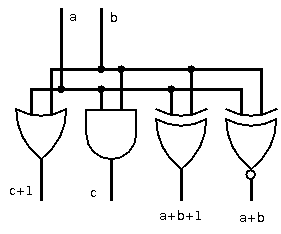
\includegraphics[width=13cm]{circuit_1.png}
    \item[c)]
        Zeigen Sie, dass sich die Kosten des modifizierten Addierers $MADD_n$ mit $O$($n$log$n$) absch�tzen lassen.
        -> Mail wegen: Kosten normaler Addierer + Modifikation (?)
    \item[d)] Erweiterungen am $MADD_n$-Addierer n�tig f�r eingangs�bertragung $c_{-1}$, Skizze Schaltkreis.

\end{itemize}


\section*{Aufgabe 2}
\begin{itemize}
    \item[a)] [Schaltkreis 2] \\
	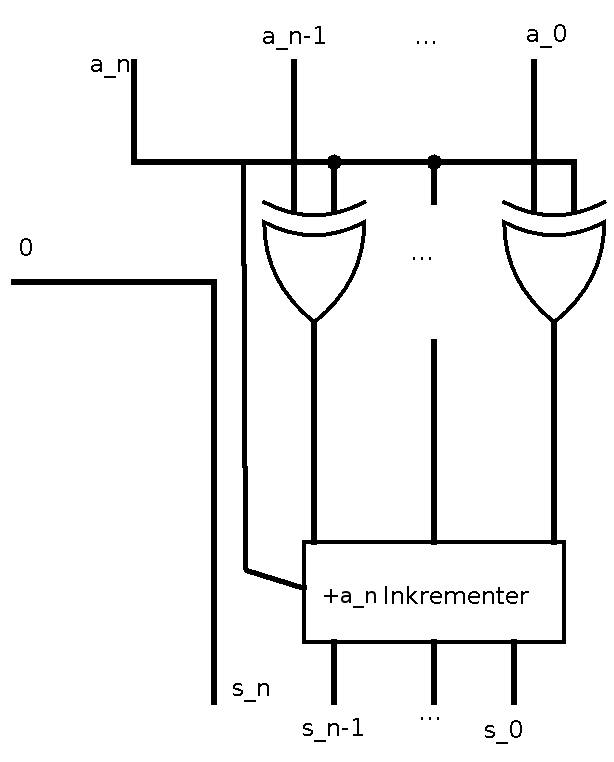
\includegraphics[width=13cm]{circuit_2.png}
    \item[b)] [Schaltkreis 3] \\
        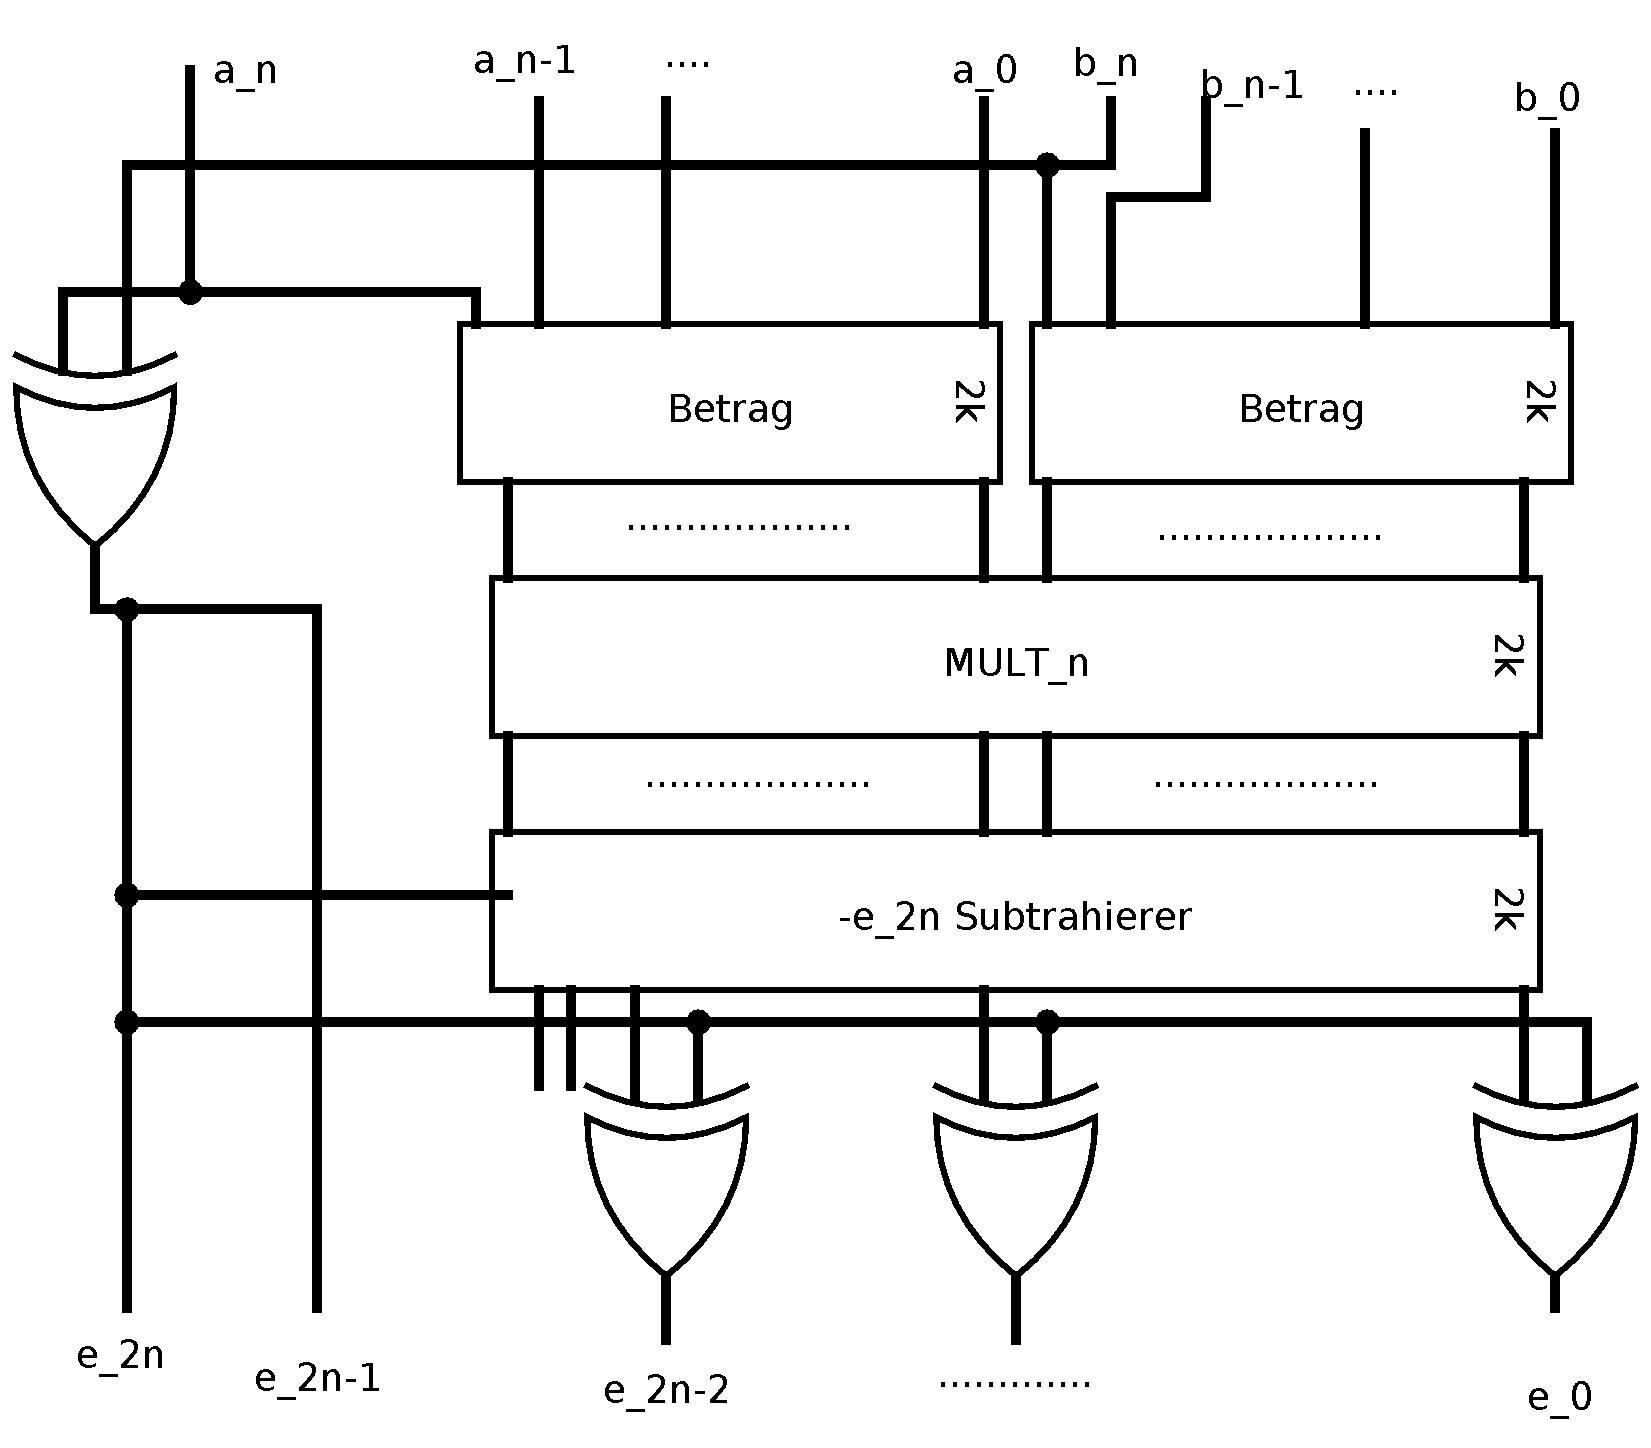
\includegraphics[width=14cm]{circuit_3.png}
        Es wird von beiden Zahlen jeweils der Betrag gebildet (s. Aufgabe a) und miteinander
        Multipliziert. Gleichzeitig wird das Vorzeichen berechnet und falls das Ergebnis negativ ist,
        wird im Folgenden die 2er-Komplement-Zahl Negiert. Die ersten Zwei bits nach dem Subtrahieren
        (von 0 bei Positivem Ergebnis) werden im Folgenden ignoriert, da wir uns sicher sein K�nnen
        dass diese die selben Werte h�tten wie unser Vorzeichen. (Hintergrund: 
        die Multiplizierte Zahl ist genau $2n - 2$ lang, die resultierenden Nuller w�rden bei
        Negativem Vorzeichen umgedreht werden, andernfalls nicht.)


\end{itemize}

\section*{Aufgabe 3}
\begin{itemize}
    \item[a)]
	\begin{tabular}{ll|ll}
		a & b & c & d\\ \hline
		1 & 1 & 0 & 0\\
		0 & 1 & 1 & 0\\
		1 & 0 & 0 & 1\\ 
		0 & 0 & 1 & 0\\
		0 & 0 & 0 & 1\\
	\end{tabular}\\\\

    \item[b)] Gehalten wird bei $a = b = 0$, gespeichert wird mit entweder $b = 1$ oder $a = 1$
        ($c = 1$ bzw. $d = 1$ und das adnere jeweils $0$) und dem anderen ($a,b$) $0$.
    \item[c)] Die schaltung ist active-high, da durch anheben der Spannung (in einem Eingang)
        ein Zustand gespeichert (gehalten) wird. 'Flackern' tritt auf beim �bergang von
        $a = b = 1$ nach $a = b = 0$. 
    \item[d)] Die Belegungen $a = b = 1$, sowie eine Zuweisende Belegungen machen l�ngerfristig
        betrachtet (au�er eine kurzzeitig Zuweisende Belegung zum Belegen) keinen Sinn, da man
        dadurch nicht eine 'abgespeicherte' Information abfragt.
        (Au�er m�glicherweise bei $a = b = 1$, man erf�hrt zumindest dass momentan nichts
        gespeichert ist.)


\end{itemize}

\end{document}
